\chapter{Spielekonsole}
\textbf{Verfasser:innen:} \\
Abatielos, Loukas (labatielos@stud.hs-bremen.de) \\
Planitz, Thalea (tplanitz@stud.hs-bremen.de) \\
Reichenberg, Lea (lreichenberg@stud.hs-bremen.de) \\
Schwanewede, Leoni (lschwanewede@stud.hs-bremen.de) \\ [1cm]

\section{Einführung}
Im zweiten Teil des Bachelorprojektes haben wir mit dem Computermuseum in Oldenburg zusammengearbeitet, um mögliche Ausstellungsobjekte zu entwickeln, die dort dauerhaft gezeigt werden können. Dabei entschieden wir uns, eine kleine Spielekonsole zu entwerfen, die den gesamten Ablauf der Datenübertragung – vom Controller über die Verarbeitung der Eingaben bis zur Weiterleitung an den Bildschirm – mithilfe von Lichtern visualisiert. Auf diese Weise wird ein Prozess sichtbar gemacht, der im Alltag normalerweise vollständig im Verborgenen abläuft und für Besucherinnen und Besucher sonst kaum greifbar wäre. \\

Spielekonsolen sind aus dem heutigen Alltag kaum mehr wegzudenken und bilden ein Kontrast zu den älteren Exponaten und eine Brücke zwischen der Technikgeschichte und der digitalen Unterhaltungselektronik, welche einen festen Platz in der heutigen Zeit eingenommen haben. Deshalb wollten wir der Ausstellung des Museums, in der vor allem historische Computer stehen, mit der Spielekonsole ein modernes Stück hinzufügen, welches auch zur Erklärung älterer Spielekonsolen dient. Außerdem ist es mit unserem Prototypen möglich, selbstgemachte Scratch-Spiele auf der Spielekonsole zu spielen, sodass er ebenfalls für die Scratch-Lernkurse für Kinder im Museum genutzt werden kann.


\section{Konzept}
Die grundlegende Problemstellung bei unserem Projekt bestand darin, eine immersive Erweiterung für das Museum zu bieten, welche eine möglichst große Anzahl an verschiedenen Personen und Altersgruppen anspricht. Außerdem sollte unser Projekt Wissen auf interessante und interaktive Weise vermitteln und das Verständnis für die gewählte Thematik vertiefen.

\subsection{AR-Idee}
Auf dem Weg zu unserer finalen Lösungsidee haben wir viele verschiedene Ideen durchdacht und ausgearbeitet. Zuerst planten wir eine AR-Applikation, mit welcher Besucher des Museums in Ausstellungsstücke hinein schauen können an Stellen, an welchen dies nicht so einfach ist. Dies kann man auch in Abbildung 1 sehen. Mit Hilfe eines grafischen Overlays könnten dann weitere Informationen zu den Bauteilen oder Vorgängen innerhalb des Ausstellungsstückes angezeigt werden. Umgesetzt werden sollte dies durch ein fest installiertes Tablet oder durch die Handys der Besucher. Auf diesen oder dem Tablet würde dann eine von uns entwickelte App oder Website die Applikation ausführen. Diese Idee haben wir letztendlich aber verworfen, weil eine andere Gruppe von Studierenden schon eine ähnliche Idee ausgearbeitet hatte und wir uns deshalb entschieden haben etwas anderes zu entwickeln. 
\pagebreak
\begin{figure}[h]
\centering
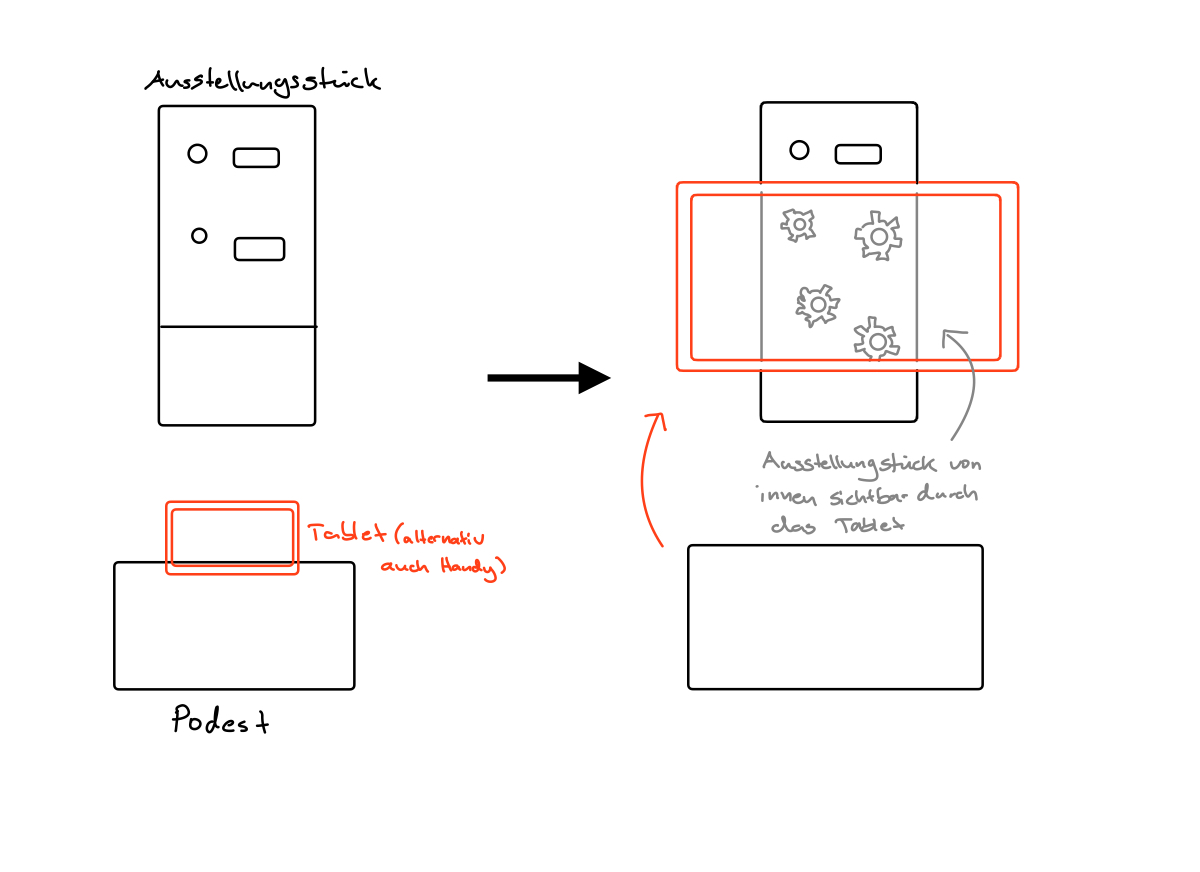
\includegraphics[width=1\textwidth]{bilder/spielekonsole/AR_Idee.jpeg} \\
\caption[Abbildung 1:]{Skizze der AR-Idee}
\end{figure}

\subsection{VR-Idee}
Unsere nächste Idee war es, mithilfe einer VR-Brille, die Funktionsweise von Virtual Reality zu erklären. Hierzu würde eine fest installierte VR-Brille ausgestellt werden, welche Besucher sich aufsetzen können. Durch diese Brille wird dann im virtuellen Raum eine Erklärung in mehreren Schritten angezeigt darüber was Virtual Reality ist und wie es funktioniert. Diese Erklärung gäbe es dann ebenfalls bildlich auf der Wand hinter unserer Station, falls Besucher aus verschiedenen Gründen keine VR-Brille aufsetzten können sollten. Der genauere Aufbau ist auch nochmal in unserer Skizze dazu in Abbildung 2 aufgezeichnet. Hier kann man auch sehen, wie die einzelnen Schritte von links nach rechts aufgezeigt werden. Bei dieser Idee kann es durchaus nötig sein, dass diese Station durchgehend von einem Mitarbeiter vom Museum unterstützt wird, weshalb wir sie später verworfen haben.
\pagebreak
\begin{figure}[h]
\centering
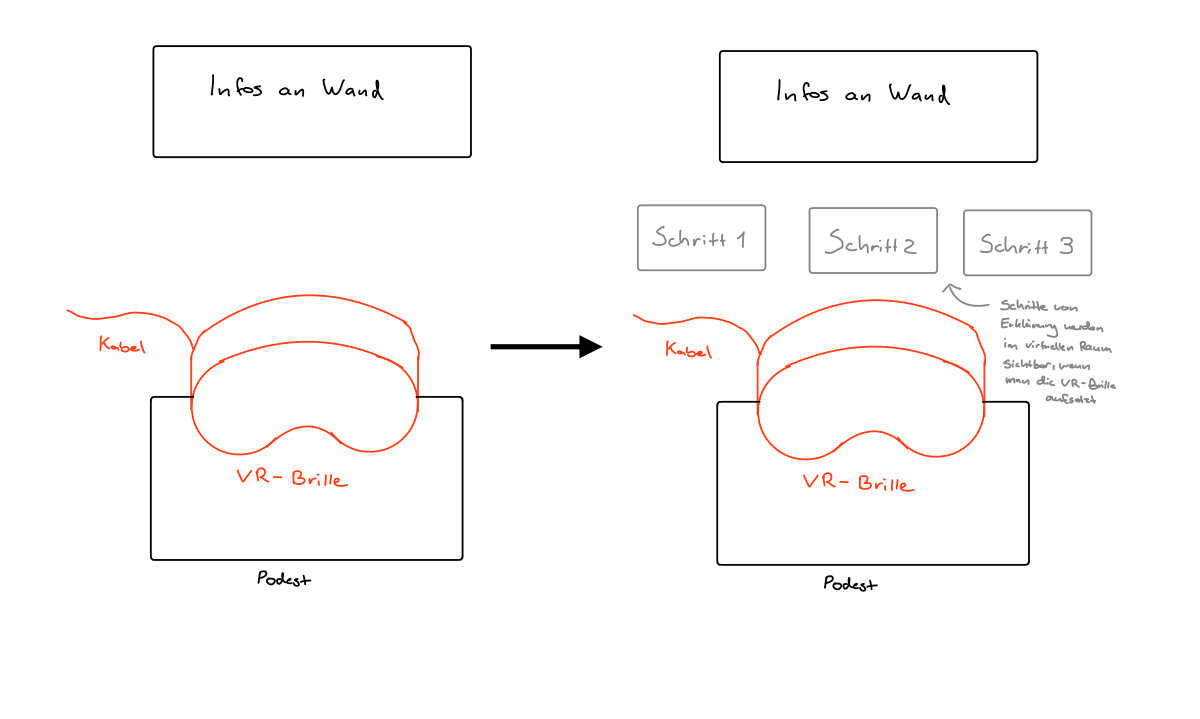
\includegraphics[width=1\textwidth]{bilder/spielekonsole/VR_Idee.jpeg} \\
\caption[Abbildung 2:]{Skizze der VR-Idee}
\end{figure}

\subsection{Spielekonsole}
Letztlich sind wir nach dem ersten Besuch im Museum auf die Idee gekommen, eine eigene Spielekonsole zu entwickeln. Inspiriert wurde diese Idee von den dort ausgestellten, alten Spielekonsolen. Der Plan war es, einen Raspberry Pi als Computer zu verwenden und diesen an einen Bildschirm anzuschließen. Für Eingaben von den Besuchern sollte ebenfalls ein Controller angeschlossen werden. Das Ziel ist es, durch selbst programmierte Spiele den Besuchern näherzubringen, wie eine Spielekonsole eigentlich funktioniert, aus welchen Komponenten sie besteht und wie diese miteinander kommunizieren. Um die Kommunikation zu verdeutlichen gibt es außerdem noch eine Lichterkette, die mit verschieden blinkenden LEDs den Informationsaustausch zwischen Controller, RaspberryPi und Bildschirm simulieren soll. Zum Ansprechen der Lichterkette verwenden wir deshalb außerdem noch einen Microcontroller. Auch hier ist der genauere Aufbau unserer Idee als Skizze in Abbildung 3 zu erkennen.
\clearpage
\begin{figure}[h]
\centering
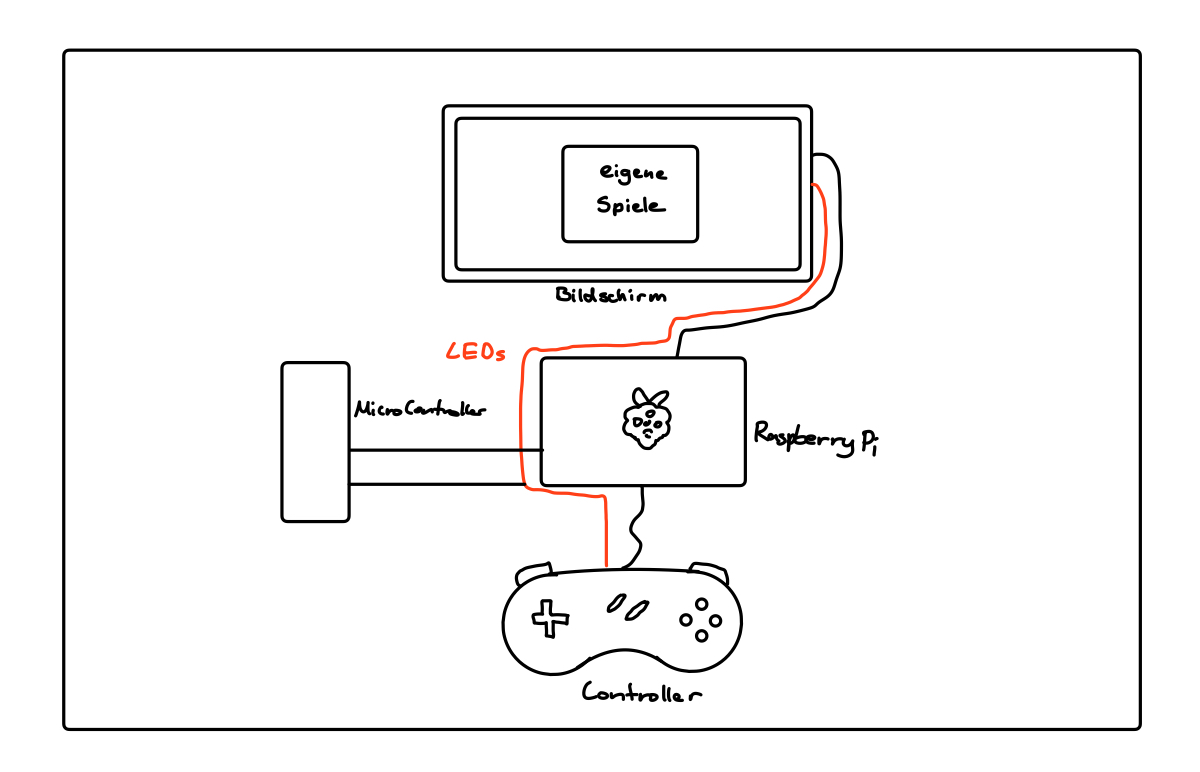
\includegraphics[width=1\textwidth]{bilder/spielekonsole/Spielekonsole_Idee.jpeg} \\
\caption[Abbildung 3:]{Skizze der Spielekonsolenidee}
\end{figure}
Um das Erweitern der Spielbibliothek zu erleichtern, soll es möglich sein, neue Spiele einfach nur in den Spiele-Ordner auf dem USB-Stick von dem Raspberry Pi zu legen. Diese sollen dann, wie abgebildet in Abbildung 4, direkt bei dem nächsten Start der Konsole in dem Menü angezeigt werden und auch auswählbar sein. Eine Höchst- oder Mindestanzahl an Spielen soll es dabei nicht geben.
\clearpage
\begin{figure}[h]
\centering
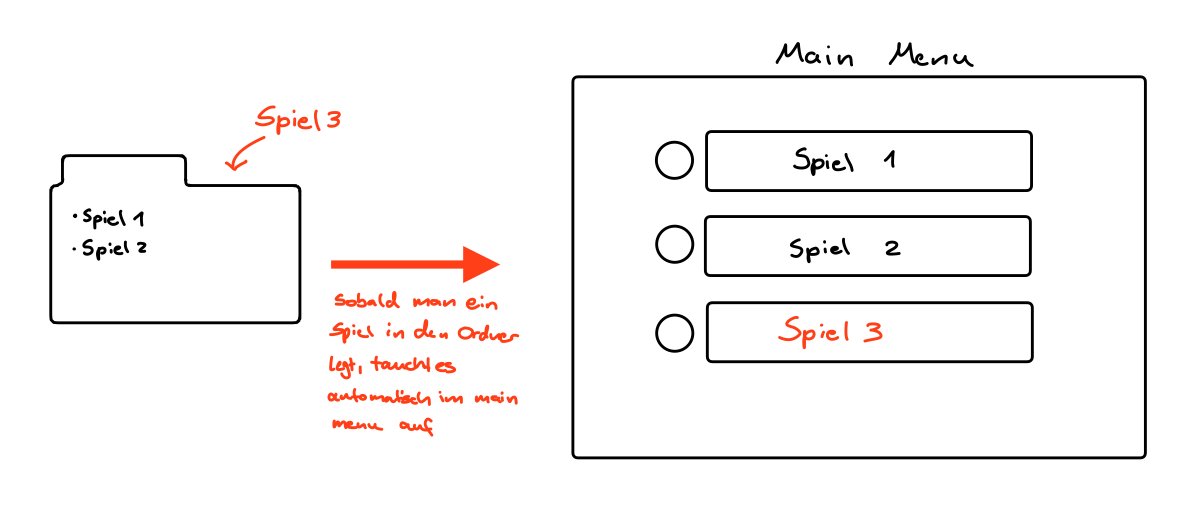
\includegraphics[width=1\textwidth]{bilder/spielekonsole/Importieren.jpeg} \\
\caption[Abbildung 4:]{Skizze zum Einbinden von neuen Spielen}
\end{figure}
Ein weiteres Ziel war es das Menü so übersichtlich wie möglich zu gestalten. Dazu haben wir vier verschiedene Versionen entworfen, welche in Abbildung 5 zu sehen sind. In der ersten Version sind die Spiele von oben nach unten angeordnet, aber anders als in allen anderen Versionen werden hier keine Thumbnails von den Spielen angezeigt. Ähnlich dazu, sind bei der zweiten Version die Spiele von links nach rechts angeordnet. Bei beiden soll man mit dem Controller jeweils durch die Spiele scrollen können. Die dritte und vierte Version sind im Gegensatz zu den ersten beiden Versionen an einem Karussell orientiert. Bei der dritten Version scrollt man durch die Spiele von links nach rechts oder auch von rechts nach links. Dabei wird das jeweilige ausgewählte Spiel in der Mitte des Bildschirms angezeigt. Bei der vierten Version besteht der einzige Unterschied zu der dritten darin, dass man hier vertikal durch die Spiele scrollen muss. \\
Am Ende haben wir uns für die dritte Version als Menü entschieden, da hier das ausgewählte Spiel im Vordergrund steht, wodurch man besser sehen kann um was für ein Spiel es sich handelt. Außerdem ist das horizontale Scrollen durch die Spielgalerie für einen horizontal breiteren Bildschirm besser geeignet.

\clearpage
\begin{figure}[h]
\centering
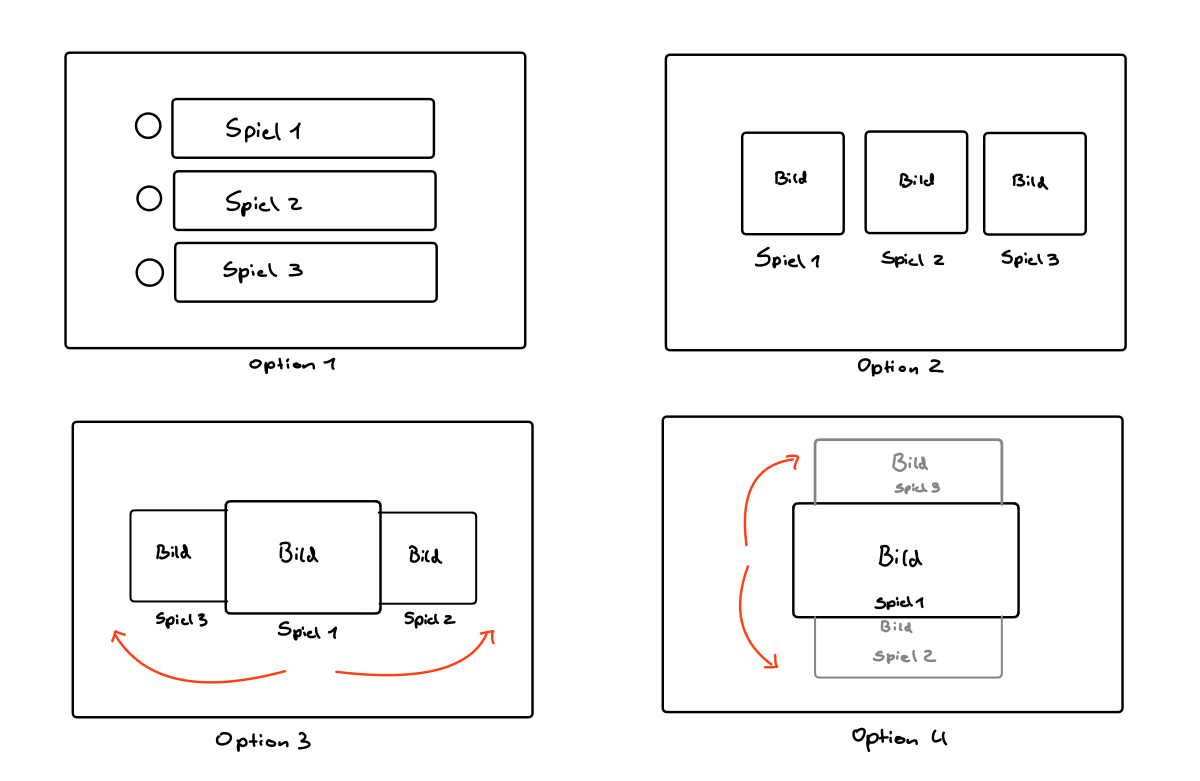
\includegraphics[width=1\textwidth]{bilder/spielekonsole/MainMenu.jpeg} \\
\caption[Abbildung 5:]{Skizze von verschiedenen Versionen des Menüs}
\end{figure}

\section{Anforderungen}
Um die Spielekonsole und ihre Funktionen umzusetzen, mussten wir sowohl technische als auch inhaltliche Anforderungen berücksichtigen. In diesem Kapitel werden alle Anforderungen, sowie ihr Verwendungszweck genannt.

\subsection{Software und Bibliotheken}
Für die Umsetzung der Spiellogik wurde Python in Kombination mit der Bibliothek Pygame verwendet (\url{https://www.pygame.org/docs/}), die grundlegende Funktionen für Spielentwicklung wie Grafikausgabe, Ereignisverarbeitung und Kollisionserkennung bereitstellt. Für die Kommunikation zwischen dem Raspberry Pi kam zusätzlich die Bibliothek PySerial (\url{https://www.pyserial.com/docs}) zum Einsatz. \\

Als Basis für die Umwandlung von Scratch-Projekten zu Python-Code haben wir das Open-Source-Projekt von sb3topy verwendet (\url{https://github.com/BirdLogics/sb3topy}), das als Ausgangspunkt für unseren eigenen Compiler genutzt wurde und für die Umwandlung in unser konsoleneigenes Spielformat erweitert wurde.\\

Für die Entwicklung wurde PyCharm (\url{https://www.jetbrains.com/pycharm/}) als Entwicklungsumgebung genutzt. Für die Steuerung der Lichterkette und des Lichtrings über den Raspberry Pico haben wir MicroPython benutzt (\url{https://micropython.org/}), da das speziell für den ressourcenschonenden Betrieb auf Mikrocontrollern ausgelegt ist. Als Betriebssystem für den Raspberry Pi kam die Desktop-Version von Raspberry Pi OS zum Einsatz (\url{https://www.raspberrypi.com/software/operating-systems/}), um sowohl den vollständigen Funktionsumfang für die Spielausgabe als auch einfache Wartung und Fehlersuche zu ermöglichen.

\subsection{Hardware}
Für den Aufbau der Konsole haben wir folgende Hardware genutzt:\\
\begin{itemize}
	\item \textbf{Raspberry Pi 4} - Der Einplatinencomputer dient als zentrale Recheneinheit für Spiellogik und Bildausgabe.
	\item \textbf{Raspberry Pico} - Ein Mikrocontroller, welcher zur Ansteuerung der NeoPixel-Lichterkette sowie des Lichtrings verwendet wird.
	\item \textbf{NeoPixel-Lichterkette} - Die Lichterkette unterstützt die Visualisierung der Datenübertragung vom Controller zur Konsole sowie von der Konsole zum Bildschirm.
	\item \textbf{Lichtring} - Der Lichtring ist angebracht auf dem Raspberry Pi, um die interne Datenverarbeitung innerhalb der Konsole zu verdeutlichen.
	\item \textbf{Bildschirm (800x480)} - Dieser kleine Bildschirm dient zur Darstellung des eigentlichen Spielgeschehens.
	\item \textbf{Nintendo SNES Controller} - Der Controller erlaubt die Steuerung von dem Menü und den Spielen.
	\item \textbf{Gehäuse (Kiste)} - Eine durchsichtige Plastikbox mit selber gebohrten Löchern für Kabel, welche als äußere Hülle der Konsole fungiert.
	\item \textbf{Verkabelung} - Die Kabel verbinden die einzelnen Komponenten untereinander und übertragen Strom, sowie auch Daten.
\end{itemize}

\subsection{Inhaltliche Anforderungen}
Neben den technischen Voraussetzungen mussten wir uns auch mit  verschiedene inhaltlichen Elementen auseinandersetzen, damit wir die nötigen Kompetenzen erwerben konnten um unser Projekt umzusetzen:
\begin{itemize}
	\item \textbf{Importieren von Dateien zur Laufzeit} - Damit nicht bei jeder neuen Spieldatei das Hauptprogramm geöffnet werden muss um den Import anzugeben, musste recherchiert werden, wie die Dateien zu der Laufzeit importiert werden können, indem das Hauptprogramm durch den Spielordner läuft und alle dort vorhandenen Spieldateien selbst importiert.
	\item \textbf{Umwandlung von Scratch-Projekten zu Python-Dateien} - Um zu ermöglichen, dass die Schüler, welche im Museum an Scratch-Kursen teilnehmen, ihre Scratch-Spiele am Ende auch auf unserer Spielkonsole spielen können, mussten wir uns damit auseinandersetzten, wie man einen Converter hierfür schreibt, bzw. schon existente Converter auf unseren Use Case anpasst. 
\end{itemize}

\section{Entwicklungsprozess}
Die Entwicklung des Prototypen verlief weitestgehend reibungslos und es gab weder große Setbacks, noch langanhaltende Probleme. 

Nach den anfänglichen Schwierigkeiten bei der Ideenfindung, bei welcher wir uns schlussendlich für die Spielekonsole entschlossen haben, ging es in die konkretere Planung der Umsetzung. Die Hochschule stellte sämtliche benötigte Hardware zur Verfügung, unter anderem den Raspberry Pi, auf welchem wir RetroPie (\url{https://retropie.org.uk/}) installierten. Dies diente dazu, auszutesten wie man Spiele auf dem Raspberry Pi in Verbindung mit einem Controller spielen kann. \\

Danach begann ein paralleler Entwicklungsprozess, wobei sich ein Teil der Gruppe auf die Software konzentrierte und der andere Teil sich um die Hardware kümmerte. Bei der Software wurden sowohl Breakout, als auch SpaceInvaders selber in Python mithilfe von Pygame programmiert als Demospiele für die Konsole. Dazu wurde das Raspberry Pi OS auf die SD-Karte installiert, um diese Spieldateien auch ausführen zu können. Auch das Menü wurde in mehreren Schritten entwickelt. Eine Schwierigkeit hier bestand darin, dass die Scripte der Spieldateien erst zu der Laufzeit importiert werden konnten, um zu gewährleisten, dass nicht jedes Mal nach dem Einfügen eines neuen Spiels, die Menü-Datei angepasst werden muss. Gelöst wurde das Problem dadurch, dass das Hauptprogramm nun bei jedem Start auflistet, welche Spieldateien momentan im Ordner liegen und diese dann zur Laufzeit importiert. Ein Bildschirmschoner wurde zu dieser Zeit ebenfalls eingebunden für den Attract Mode.\\
Gleichzeitig wurde bei der Hardware die Steuerung der Lichterkette und des Lichtrings implementiert, welche jeweils Leuchtimpulse senden, ausgelöst von den Eingaben auf dem Controller. Gesteuert wird dieser Prozess über den Mikrocontroller, bei welchem es von Zeit zu Zeit immer mal wieder Probleme bei der Erreichbarkeit gab. Diese lassen sich jedoch durch das Aus- und Wiedereinstecken des Mikrocontrollers am Raspberry Pi beheben. Später traten ebenfalls Schwierigkeiten mit der Verlötung der einzelnen Kabel am Mikrocontroller auf, da niemand aus unserer Gruppe zuvor viel Erfahrung mit dem Löten gesammelt hatte und einige Kabel dadurch einen Wackelkontakt aufwiesen. Auf Grund dessen kam es immer wieder zu Ausfällen der Beleuchtung des Lichtrings. Anfangs leuchtete der Lichtring gar nicht mehr auf, was aber mit einem weiterem Löttermin behoben wurde. Dennoch kommt es gelegentlich zu einem Wackelkontakt bei dem Kabel an dem der Lichtring angeschlossen ist, weshalb er dann nicht aufleuchtet.\\

In den letzten Schritten erweiterten wir die Software unseres Prototypen noch um die Möglichkeit Scratch-Projekte in Python-Dateien umzuwandeln auf Nachfrage des Museums. Damit ist es nun auch möglich selbstgemachte Scratch-Spiele auf unsere Spielekonsole zu spielen. Das letzte große Problem bei dem Entwicklungsprozess unseres Prototypen stellte die klare Definition und Umsetzung des Lernziels für Besucher des Museums dar. Nach einer Woche entschlossen wir uns letztendlich den genaueren Ablauf der Kommunikation der einzelnen Komponenten, welcher schon vorher durch die LEDs simuliert wurde, durch eine kurze Erklärung vor jedem Spiel zu unterstützen.  Wir platzierten ebenfalls unseren Prototypen in einer durchsichtigen Plastikbox zum Schutz und fügten nach dem finalen Feedback im letzten Labor noch das Logo der Hochschule ein.
\clearpage

\section{Prototyp}
Der entwickelte Prototyp ist eine Spielkonsole, die auf einem Raspberry Pi basiert. Die Spielkonsole dient dazu, den Ablauf zwischen den Hardware-Komponenten anschaulich darzustellen, wenn beispielsweise ein Spiel gespielt wird, und allgemein das Interesse an Hardware zu erwecken. Um die Zusammenarbeit der Hardware-Komponente zu zeigen, wurde eine transparente Box als Behälter ausgesucht. Außerdem ermöglicht der Prototyp Schülern, welche einen Scratch-Kurs im Museum besuchen, ihre fertigen Projekte auf der Spielekonsole zu spielen, indem die Scratch-Projekte in Spieldateien in Python umgewandelt werden können. 

\subsection{Bestandteile der Spielkonsole}
Die Kernkomponente des Prototyps ist der Raspberry Pi, welchen man auf Abbildung 6 als kleinen schwarzen Kasten in der Mitte des Bildes erkennen kann. Er ist ein Einplatinencomputer und führt die Python-Scripte aus. Ebenfalls verarbeitet er die Nutzereingaben und steuert daraufhin den Mikrocontroller an. Auf dem USB-Stick, welcher hinten an dem Raspberry Pi angeschlossen ist, liegen alle wichtigen Dateien, unter anderem auch die Spieldateien. \\
Der Mikrocontroller befindet sich links von dem Raspberry Pi in der Abbildung 6. Er steuert sowohl die Lichterkette als auch den Lichtring und sorgt für die Lichtimpulse, welche die Datenübertragung simulieren sollen. Die Kabel sind fest an den Mikrocontroller angelötet.\\
Über dem Raspberry Pi befindet sich der Bildschirm auf dem alle Spielinhalte, sowie das Menü angezeigt werden. Mit einer Auflösung von 800x480 ist er ein relativ kleiner Bildschirm, welcher für unseren Prototypen jedoch völlig ausreichend ist.\\
Unter dem Raspberry Pi liegt der SNES Controller, welcher durch ein Loch mit dem Raspberry Pi verbunden ist, sodass er weiterhin erreichbar bleibt, auch wenn der Deckel der Box geschlossen wird. Da der Anschluss für den Controller auf der Hinterseite des Raspberry Pis liegt, führt das Kabel unter diesem lang, um den Gesamtaufbau übersichtlicher zu gestalten.\\
Sowohl die Lichterkette, als auch der Lichtring sind für die Veranschaulichung der Datenübertragung zwischen den einzelnen Komponenten verantwortlich. Beide sind an den Mikrocontroller links angeschlossen. Die Lichterkette verläuft von der Stelle an der das Kabel des Controllers auf die Box trifft, unter dem Raspberry Pi lang bis hin zu dem Bildschirm. Vor dem Raspberry Pi zeigt sie die Datenübertragung des Controllers an und nach dem Raspberry Pi die Datenübertragung zum Bildschirm. Der Lichtring sitzt auf dem Raspberry Pi und zeigt die Verarbeitung der Daten im Raspberry Pi selbst an.\\
Von der transparenten Box, welchen den Prototypen selber schützt, lässt sich in Abbildung 6 nur der Boden sehen, da hier der Deckel entfernt wurde um die einzelnen Komponenten klarer darstellen zu können. Wenn der Deckel geschlossen ist, sitzt der Bildschirm auf dem Deckel der Box. 
\begin{figure}[h]
	\centering
	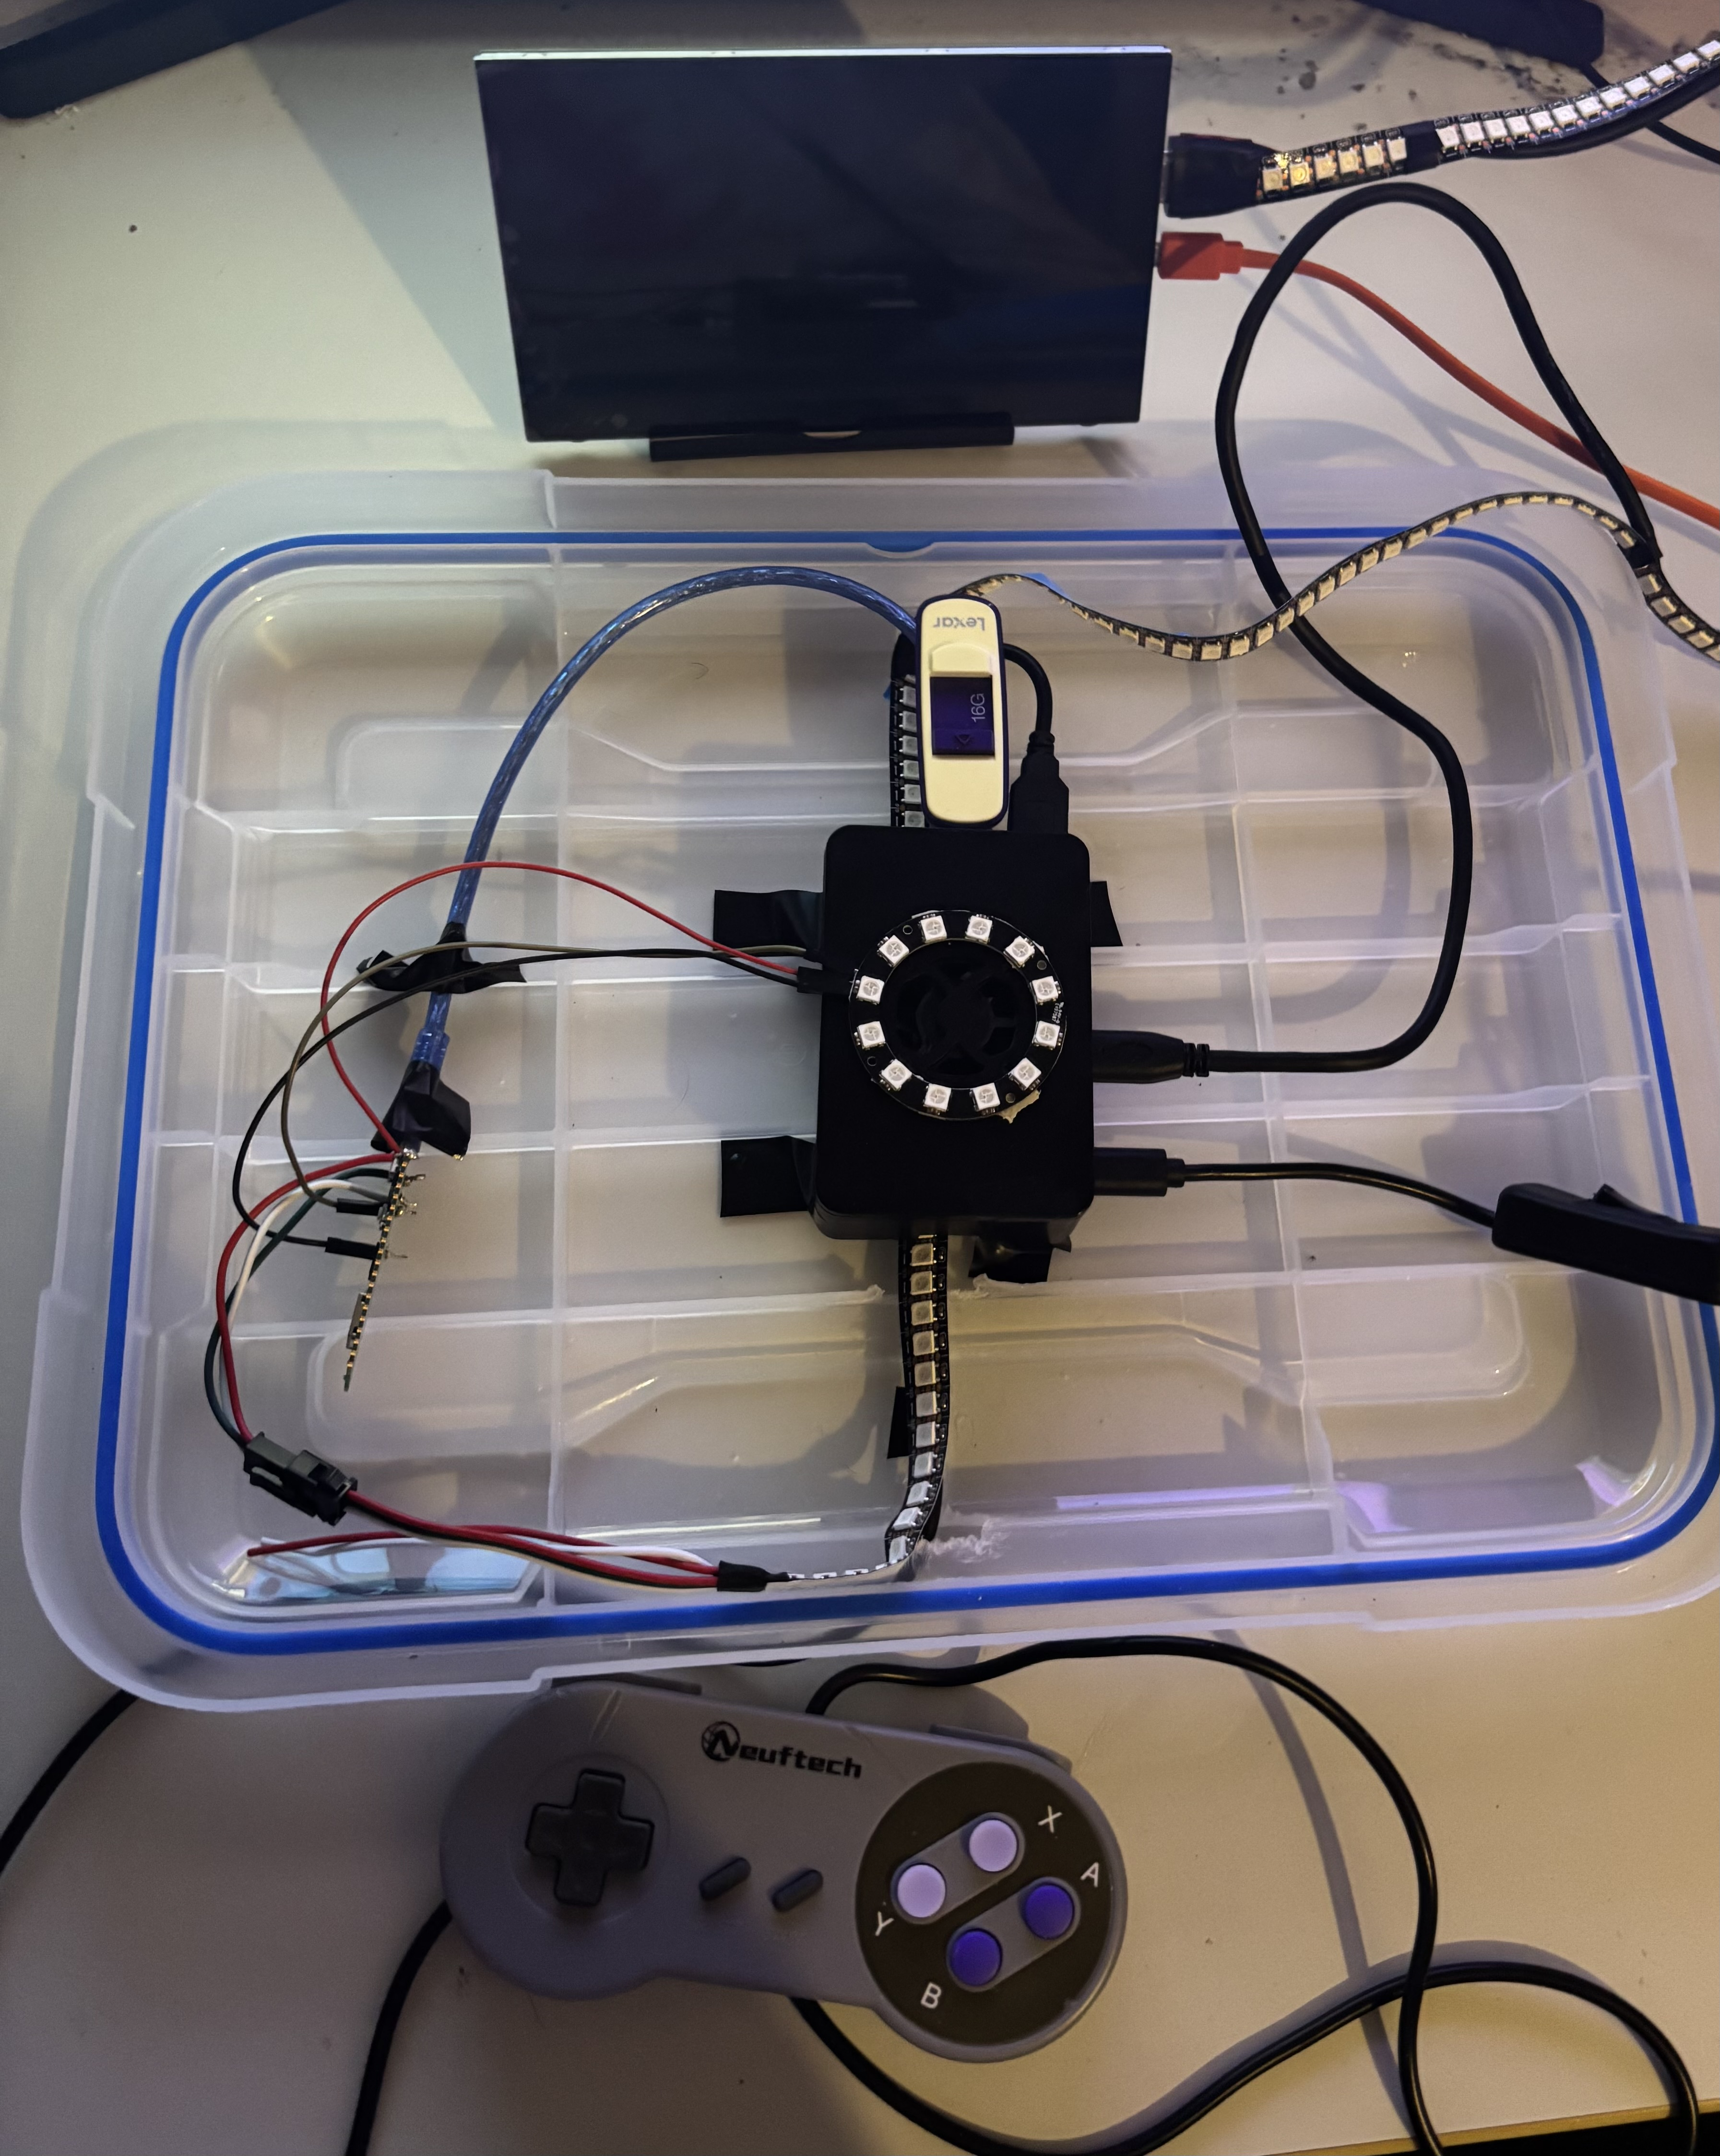
\includegraphics[width=0.7\textwidth]{bilder/spielekonsole/Spielekonsole.jpeg} \\
	\caption[Abbildung 6:]{Aufbau der Spielkonsole}
\end{figure}

\subsection{Menü}
Bei dem Starten der Spielkonsole wird zuerst des Menü angezeigt, welches man in Abbildung 7 sehen kann. Hier werden drei der vorhandenen Spiele in der Spielbibliothek abgebildet. Das in der Mitte des Bildschirms liegende Spiel zeigt dabei das aktuell ausgewählte Spiel an. Dieses lässt sich über Drücken der 'A'-Taste auf dem Controller öffnen. Um ein anderes Spiel auszuwählen kann der Nutzer sich mit der linken und rechten Pfeiltaste auf dem Controller durch die Spielbibliothek klicken. Wenn man sich lange genug in eine Richtung klickt, so kommt man irgendwann wieder bei dem Anfangsspiel an, da das Menü an einem Karussell inspiriert ist. Es gibt hierbei weder eine benötigte Mindestanzahl, noch Höchstanzahl an Spielen die man auf den USB-Stick legen muss.\\
Um ein neues Spiel zu der Spielkonsole hinzufügen, genügt es dieses in den dafür vorgesehenen Ordner auf dem USB-Stick zu legen. Das Python-Skript des Menüs geht zu beginn der Anwendung durch alle Spieldateien im Ordner durch und importiert diese dann während der Laufzeit, sodass das manuelle Importieren einer neuen Spieldatei auf dem Hauptskript nicht mehr notwendig ist um die Benutzerfreundlichkeit unseres Prototypen zu erhöhen. 
\begin{figure}[h]
	\centering
	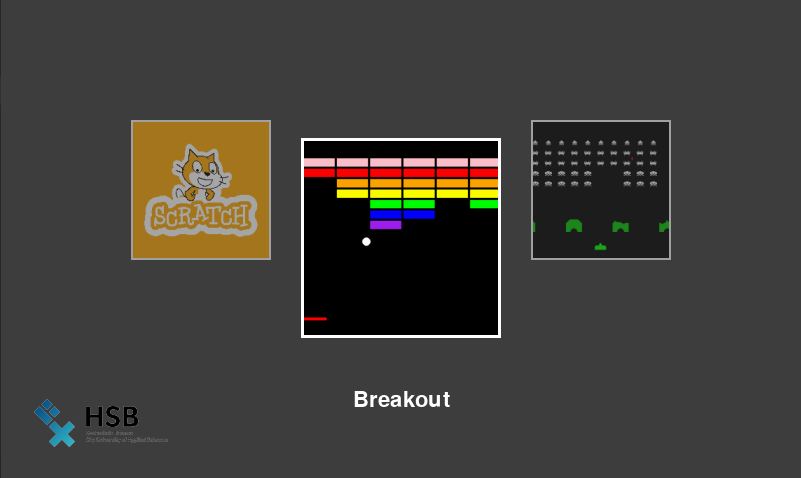
\includegraphics[width=1\textwidth]{bilder/spielekonsole/Menü.PNG} \\
	\caption[Abbildung 7:]{Menü}
\end{figure}
\clearpage

\subsection{Spiele mit Python}
Unser Prototyp besitzt sowohl Breakout, als auch Space Invaders, welche jeweils selber programmiert sind. Es ist aber auch möglich eigene Spiele, welche mit Pygame programmiert wurden, einzufügen. \\
In Abbildung 8 ist unsere Version von Breakout abgebildet. Links oben befindet sich der aktuelle Score des Spielers und rechts oben die Anzahl der noch vorhandenen Leben. Ziel des Spiels ist es alle bunten Blöcke zu zerstören, indem man den Ball im richtigen Winkel von dem kleinen Rechteck unten abprallen lässt. Dieses rote Rechteck kann der Spieler nach links und rechts bewegen. Sollte der Ball den unteren Rand unterhalb des roten Rechtecks treffen, so verliert der Spieler ein Leben und der Ball wird wieder in der Mitte des Spielfelds platziert. Sollte der Spieler alle seine Leben verloren haben, so beginnt das Spiel sofort neu, da es sich hier nur um ein Demospiel handelt.
\begin{figure}[h]
	\centering
	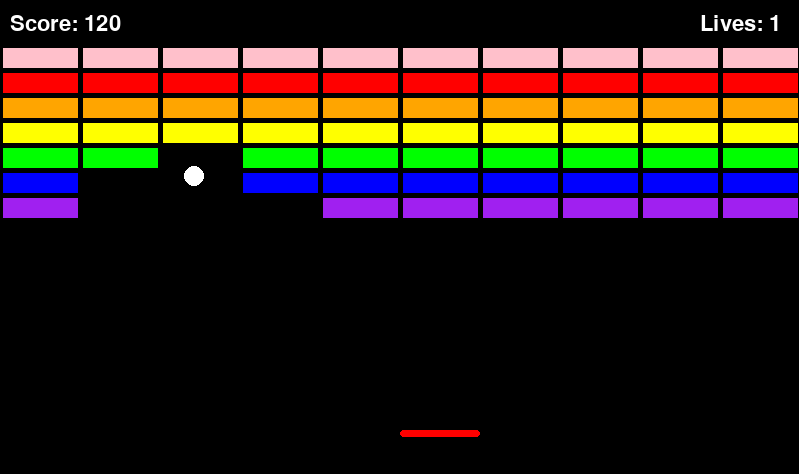
\includegraphics[width=01\textwidth]{bilder/spielekonsole/Breakout.PNG} \\
	\caption[Abbildung 8:]{Breakout}
\end{figure}
\clearpage
Das andere vorgefertigte Spiel ist Space Invaders, welches in Abbildung 9 gezeigt wird. Hier kann der Spieler ebenfalls seinen Score in der linken oberen Ecke sehen und de Anzahl seiner noch vorhandenen Leben in der rechten oberen Ecke. Der Spieler selbst befindet sich zu Anfang des Spiels ganz unten als grüne Figur in der Mitte. Das Ziel ist es die Gegner, welche in weiß in der Mitte des Bildschirms zu finden sind, abzuschießen. Dafür kann sich der Spieler nach links und rechts bewegen und mit dem 'A'-Knopf auf dem Controller schießen. Leben verliert er indem er von den Angriffen der Gegner getroffen wird, vor welchen er sich allerdings auch schützen kann indem er Schutz unter den größeren, grünen Figuren über sich sucht. Die Gegner bewegen sich nach links und rechts während des Spiels und kommen dem Spieler immer näher. Wenn er alle Gegner getroffen hat, dann erscheinen neue in der Spielmitte. Verliert er alle Leben, fängt das Spiel sofort wieder neu an, da es sich auch hier nur um eine Demoversion handelt. 
\begin{figure}[h]
	\centering
	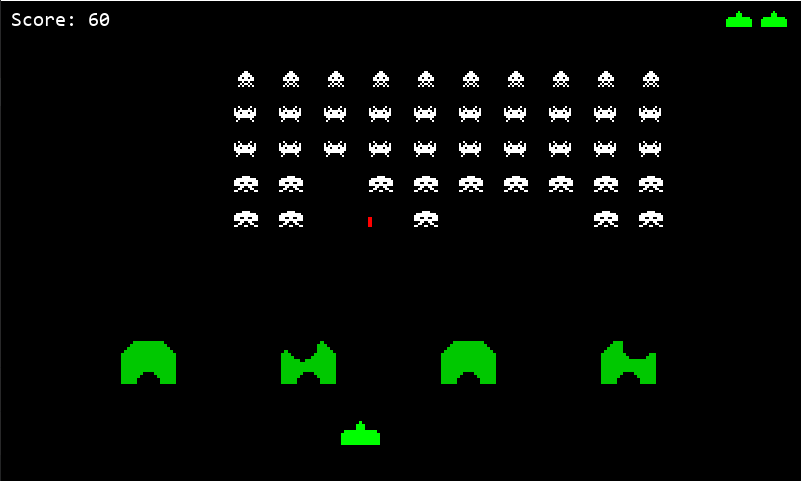
\includegraphics[width=1\textwidth]{bilder/spielekonsole/SpaceInvaders.PNG} \\
	\caption[Abbildung 9:]{Space Invaders}
\end{figure}
\clearpage
Eigene Spiele, welche man mithilfe von Pygame programmiert hat kann man in den Spielordner auf dem USB-Stick legen. Die Spiele benötigen einen Namen, ein Thumbnail von der Größe 200x200 und die Spiellogik muss ein einer Methode namens 'run()' liegen, damit sie in dem Menü angezeigt und ausgewählt werden können. Alle Spiele kann man außerdem mit drücken von 'Select' verlassen um in das Menü zurückzugelangen. Die Anwendung der Spielkonsole schließt man, indem man in dem Menü 'Select' drückt.

\subsection{Spiele mit Scratch}
Zusätzlich besteht die Option eigene, mit Scratch entwickelte Spiele, der Spielbibliothek hinzuzufügen. Diese muss man zuerst mit unserem Converter in eine Python-Datei umwandeln und kann sie anschließend in den Spielordner auf dem USB-Stick legen. Dieser Converter basiert auf sb3topy (\url{https://github.com/BirdLogics/sb3topy}) und wurde in unserem Prototypen noch leicht erweitert, um an unsere Anforderungen angepasst zu sein. Danach taucht das Scratch-Spiel in dem Menü mit dem Scratch-Logo als Thumbnail auf und kann gespielt werden. Testweise wurden selbst ein paar Scratch-erstellte Spiele umgewandelt und hinzugefügt. Eines davon lässt sich in Abbildung 10 mit dem Scratch-Logo als bewegbare Figur sehen.\\
Die Möglichkeit auch Scratch-Spiele auf der Spielkonsole spielen zu können wurde auf Nachfrage des Museums eingebaut, damit Schüler, die im Oldenburger Computermuseum einen Scratch-Kurs besuchen, am Ende ihre Spiele auch auf einer richtigen Spielkonsole spielen können. 
\begin{figure}[h]
	\centering
	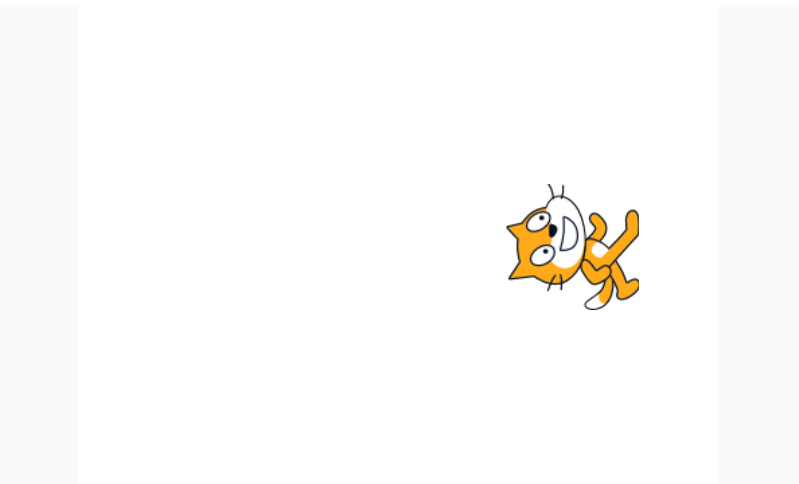
\includegraphics[width=0.8\textwidth]{bilder/spielekonsole/Scratch.PNG} \\
	\caption[Abbildung 10:]{Erstelltes Spiel mit Scratch}
\end{figure}
\clearpage


\subsection{Attract Mode}
Der Attract Mode besteht aus zwei Bestandteilen. Zum einem aus dem Bildschirmschoner, welcher nach 20 Sekunden Inaktivität anspringt und in Abbildung 11 zu sehen ist. Er zeigt eine Demoversion eines Spiels und fordert den Besucher dazu auf den 'A'-Knopf zu drücken, um zurück zu dem Menü zu gelangen. In der linken unteren Ecke kann man außerdem das Hochschullogo erkennen. Zum anderen besteht der Attract Mode aus dem Inaktivitätsmodus der Lichterkette, welche dann lauter Lichtimpulse zeigt, jeder einzelne mit einer zufälligen Farbe.\\
Der Attract Mode dient dazu im Fall der Inaktivität neue Museumsbesucher anzulocken und auf den Prototypen aufmerksam zu machen. Während der verschiedenen Testphasen erwies er sich darin auch als sehr erfolgreich. 
\begin{figure}[h]
\centering
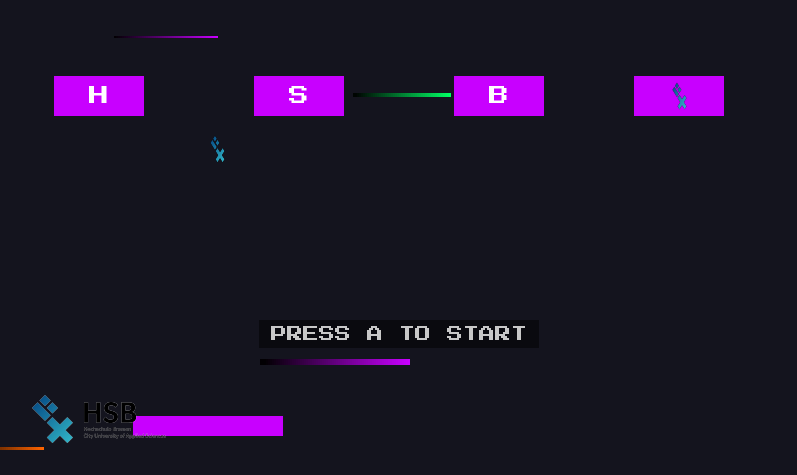
\includegraphics[width=1\textwidth]{bilder/spielekonsole/attractMode.png} \\
\caption[Abbildung 11:]{Bildschirmschoner}
\end{figure}

\subsection{Lichterkette}
Die Lichterkette ist dazu da, um die Datenübertragung zwischen den einzelnen Komponenten zu visualisieren. Erfolgen Eingaben von dem Nutzer auf dem Controller, so zeigt die Lichterkette den Weg dieser von dem Controller zu dem Bildschirm an. Der Lichtring, welche direkt auf dem Mikrocontroller sitzt, lässt dabei ein blaues Licht im Kreis laufen, um die Verarbeitung der Daten im Raspberry Pi zu visualisieren. Jede Eingabe des Nutzer wird dabei in einem eigenen Farbimpuls dargestellt. Es gibt insgesamt fünf verschiedene Farben, die aufleuchten können:
\begin{itemize}
	\item \textbf{Blau} - bei dem Drücken der 'A'-Taste
	\item \textbf{Rot} - Signal für links
	\item \textbf{Grün} - Signal für rechts
	\item \textbf{Gelb} - Signal für oben
	\item \textbf{Cyan} - Signal für unten
\end{itemize} 
Um die Zusammenhänge zwischen der Lichterkette und der Hardware zu erläutern, wurde im Prototypen eine Erklärung vor jedem Spiel eingebunden. Hier werden in drei Schritten die jeweiligen Schritte in der Datenübertragung angezeigt. In Abbildung 12 wird die Übertragung der Daten zwischen dem Controller und dem Raspberry Pi gezeigt. In Abbildung 13 sieht man eine Erklärung darüber, wie die Verarbeitung der Daten im Raspberry Pi von dem Lichtring dargestellt wird. Schlussendlich zeigt Abbildung 14 wie die Übertragung der Daten zwischen dem Raspberry Pi und dem Bildschirm auf der Lichterkette aussieht.
\begin{figure}[h]
	\centering
	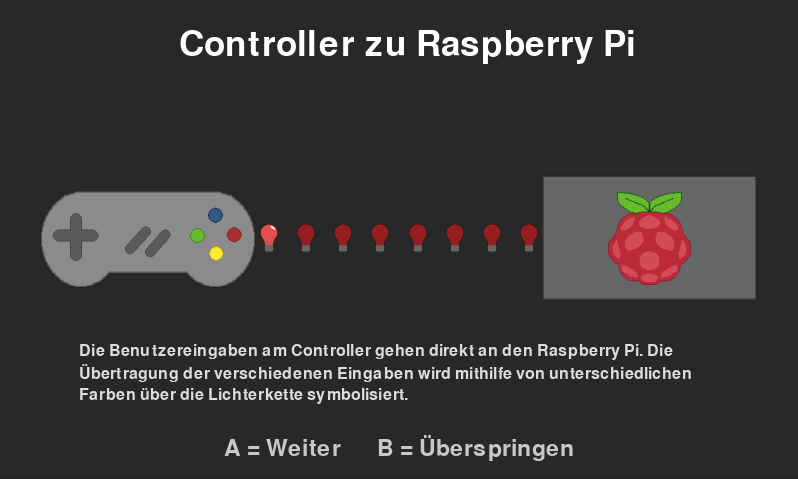
\includegraphics[width=0.8\textwidth]{bilder/spielekonsole/Tutorial1.PNG} \\
	\caption[Abbildung 12:]{Controller zu Raspberry Pi}
\end{figure}
\begin{figure}
	\centering
	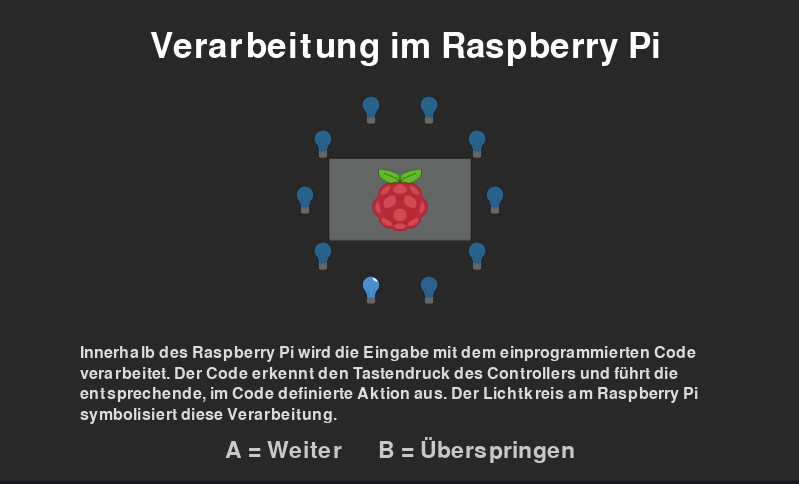
\includegraphics[width=0.8\textwidth]{bilder/spielekonsole/Tutorial2.PNG} \\
	\caption[Abbildung 13:]{Verarbeitung im Raspberry Pi}
\end{figure}
\begin{figure}
	\centering
	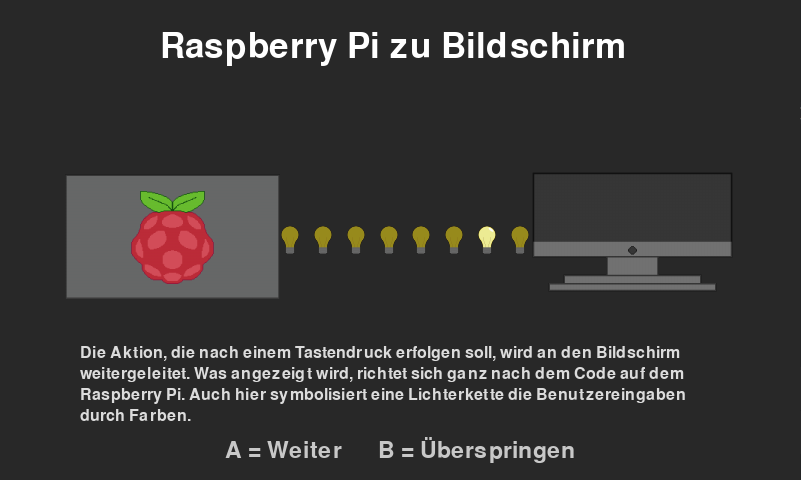
\includegraphics[width=0.8\textwidth]{bilder/spielekonsole/Tutorial3.PNG} \\
	\caption[Abbildung 14:]{Raspberry Pi zu Bildschirm}
\end{figure}
\clearpage

\section{Erprobung und Reflexion}
Bei den finalen Besprechungen im Museum sowie auch im Labor hat sich unser Prototyp als funktionsfähig und zufriedenstellend bewiesen. Er hat unseren Testern viel Spaß beim ausprobieren der Spiele bereitet und auch besonders mit dem Attract Mode Personen fasziniert. \\

\subsection{Museums Feedback}
Das Feedback des Museums fiel größtenteils positiv aus. Unsere selbst programmierten Spiele sorgten für Begeisterung und auch der Attract Mode wurde gelobt. Das Museum freute sich über die Implementierung des Scratch-zu-Python-Converters, da dieser in Verbindung mit museumseigener Scratch-Lernkursen für Kinder genutzt werden kann. Hier können die Kinder dann an unserem Prototypen ihre selbstgemachten Scratchspiele testen. \\
Zur Verbesserung wünschte sich das Museum noch eine klarere Definition davon, was wir den Besuchern mit unserem Prototypen beibringen wollen und eine klarere Ausarbeitung der Umsetzung dessen.

\subsection{Labor Feedback}
Nachdem wir noch eine kurze Zeit zum Überarbeiten unseres Prototypen hatten und dort unser Lernziel für Besucher klarer definiert und technisch umgesetzt haben, in Form von einer der kleinen Erklärung der Bedeutung der Lichterkette vor jedem Spiel, folgte das Feedback aus dem letzten Labor. \\
Hier erreichte uns nur positives Feedback. Jetzt mit der kurzen Erklärung vor den Spielen bildet unser Prototyp ein abgerundetes, funktionsfähiges und auch interaktives, zukünftiges Ausstellungsstück, welches mit seinem Attract Mode Personen anlockt, mit seinen Spielen begeistert und auch das Verständnis vom Aufbau von Spielekonsolen bei dem Besuchern des Museums stärkt.\\
Es wurde sich abschließend gewünscht, dass wir das Logo der Hochschule auf dem Bildschirm unseres Prototypen noch einbauen. Dies haben wir als letzten Schritt vor der Vollendung unseres Prototypen dann auch noch unternommen, sodass unser Prototyp nun final fertiggestellt wurde und allgemein sehr viel positives Feedback bekommen hat. 

	

\section{Resümee und Ausblick}
Im Rahmen dieses Bachelorprojektes ist ein funktionsfähiger Prototyp entstanden, der genau das macht, was wir uns zu Beginn vorgenommen hatten: Er macht den unsichtbaren Prozess der Datenübertragung – vom Computer über die Verarbeitung bis zur Ausgabe auf dem Bildschirm – für Museumsbesucher mithilfe von Lichtern nachvollziehbar sichtbar. Damit zeigen wir, dass auch komplexe Abläufe mit einfachen visuellen Mitteln verständlich vermitteln lassen, ohne das großes Vorwissen in der Informatik wichtig ist.

\subsection{Lessons Learned}
Die Spielekonsole wurde mit Python und Pygame umgesetzt. Ein besonderes Augenmerk des Kurators vom Computermuseum war ein Compiler, der Scratch-Code in Python-Code übersetzt. Dieser erste Übersetzungsschritt ließ sich vergleichsweise gut nachvollziehen und umsetzen. Allerdings erforderte der zweite Schritt: die Umwandlung der generierten Python-Datei in das Spielformat der Konsole etwas komplizierter. Da der aus Scratch generierte Code typischerweise davon ausgeht, direkt als Hauptprogramm ausgeführt zu werden, mussten wir zunächst eine Lösung dafür finden, wie sich dieser Code stattdessen sauber in der Spiellogik der Konsole einbinden lässt. Unsere entwickelte Lösung entfernt die entsprechenden Main-Bestandteile automatisch und überführt den restlichen Code, neu eingerückt, in eine run() – Funktion, die von der Konsole aufgerufen werden kann. Damit hat sich das Problem mit vergleichsweise wenig Aufwand tatsächlich lösen können, was ein Aspekt war, welcher von Beginn an nicht offensichtlich war und erst durch Ausprobieren geklärt werden konnte. \\
Gleichzeitig handelt es sich noch um einen Prototyp, wo noch nicht alle Möglichkeiten ausgeschöpft sind, die für einen dauerhaften Museumsbetrieb wünschenswert wären. Einige Punkte konnten im Rahmen des Projektes aufgrund von Zeitlichen gründen nicht mehr umgesetzt werden und bieten Stellen zur Weiterentwicklung.

\subsection{Offene To-Dos}
\begin{itemize}
	\item Die Entwicklung eines robusten, museumstauglichen Gehäuses, welches für den Dauerbetrieb im Museum besser ausgelegt ist.
	\item Das Erstellen einer Game-Over-Nachricht bei Breakout und Space Invaders.
\end{itemize}

\subsection{Weiterführende Ideen}
\begin{itemize}
	\item Der Einsatz von mehr Lichtern bzw. feinere Visualisierung, um den Datenübertragungsprozess noch detaillierter und anschaulicher zu erklären.
	\item Die Erweiterung um weiter Spiele, um die Konsole vielseitiger für wiederkehrende Besucher interessanter zu gestalten.
	\item Die Erweiterung des Scratch-zu-Pygame-Compilers, um noch mehr Scratch-Funktionen zu unterstützen und so den Schülern im Workshop noch mehr kreativen Freiraum zu lassen.
	\item Das Einbauen eines größeren Bildschirms, damit Besucher im Museum die Spiele angenehmer Spielen können.
\end{itemize}
Insgesamt zeigt das Projekt, dass mit vergleichsweise einfachen Mitteln ein anschauliches Exponat geschaffen werden kann, das die Lücke zwischen historischer und moderner Computertechnik im Museum schließt. Der entstandene Prototyp bildet somit eine gute Grundlage, auf der auch zukünftige Arbeiten, sei es im Rahmen weiterer studentischer Projekte oder durch das Museum selbst, aufbauen können, um die Spielekonsole zu einem vollwertigen, dauerhaften Ausstellungsstück auszubauen.
\clearpage

\section{Links}
\textbf{PyCharm: }\url{https://www.jetbrains.com/pycharm/} \\
\textbf{Pygame: }\url{https://www.pygame.org/docs/} \\
\textbf{PySerial: }\url{https://www.pyserial.com/docs} \\
\textbf{MicroPython: }\url{https://micropython.org/} \\
\textbf{sb3topy: }\url{https://github.com/BirdLogics/sb3topy} \\
\textbf{Raspberry Pi OS: }\url{https://www.raspberrypi.com/software/operating-systems/} \\
\textbf{RetroPie: }\url{https://retropie.org.uk/}
